\documentclass[a4paper,11pt]{book}
\usepackage{listings}
\usepackage[utf8]{inputenc}
\usepackage{titlesec}
\usepackage{fancyhdr}
\usepackage[spanish,es-tabla]{babel}
\usepackage[hidelinks]{hyperref}
\usepackage{xcolor}
\usepackage{pdfpages}
\usepackage{url}
\usepackage{booktabs}
\usepackage[export]{adjustbox}
\usepackage{fancybox}

\usepackage{tikz}
\usepackage{pgfplotstable}
\usepackage{pgfplots}

\usepackage{textcomp}

\usepackage{wrapfig}


\usepackage{float}

\usepackage{booktabs}

\usepackage{rotating}

% Información reutilizable
\newcommand{\asunto}{Inteligencia Computacional}
\newcommand{\titulo}{Problemas de optimización combinatoria QAP}
\newcommand{\grado}{Máster Profesional en Ingeniería Informática}
\newcommand{\autor}{Ernesto Serrano Collado}
\newcommand{\email}{info@ernesto.es}
\newcommand{\profesor}{Fernando Berzal Galiano}
\newcommand{\escuela}{Escuela Técnica Superior de Ingenierías Informática y de Telecomunicación}
\newcommand{\universidad}{Universidad de Granada}
\newcommand{\ciudad}{Granada}
\newcommand{\vers}{Versión 0.1}
\providecommand{\keywords}{software libre, inteligencia artificial, algoritmos evolutivos}


% Información archivo
\hypersetup{
	pdfauthor = {\autor\ (\email)},
	pdftitle = {\titulo},
	pdfsubject = {\asunto},
	pdfkeywords = {\keywords},
	pdfcreator = {MacTeX con el paquete TeX Live},
	pdfproducer = {pdflatex}
}

% Estilo de cabeceras
\pagestyle{fancy}
\fancyhf{}
\fancyhead[LO]{\leftmark}
\fancyhead[RE]{\rightmark}
\fancyhead[RO,LE]{\textbf{\thepage}}
\setlength{\headheight}{1.5\headheight}

% Redefinición de comandos
\renewcommand{\lstlistingname}{Fragmento de código}
\renewcommand{\lstlistlistingname}{Índice de fragmentos de código}
\renewcommand{\chaptermark}[1]{\markboth{\textbf{#1}}{}}
\renewcommand{\sectionmark}[1]{\markright{\textbf{\thesection. #1}}}

% Definición de colores
\definecolor{gray97}{gray}{.97}
\definecolor{gray75}{gray}{.75}
\definecolor{gray45}{gray}{.45}
\definecolor{gray30}{gray}{.94}
\definecolor{lightgray}{rgb}{.9,.9,.9}
\definecolor{darkgray}{rgb}{.4,.4,.4}
\definecolor{purple}{rgb}{0.65, 0.12, 0.82}
\definecolor{background}{HTML}{EEEEEE}
\definecolor{delim}{RGB}{20,105,176}
\colorlet{punct}{red!60!black}
\colorlet{numb}{magenta!60!black}

	\definecolor{dkgreen}{rgb}{0,0.6,0}
	\definecolor{gray}{rgb}{0.5,0.5,0.5}
	\definecolor{mauve}{rgb}{0.58,0,0.82}

% Listados
\lstset{
	aboveskip=0.5cm,
	backgroundcolor=\color{gray97},
	basicstyle=\scriptsize\ttfamily,
	breaklines=true,
	%commentstyle=\color{gray45},
	frame=Ltb,
	framerule=0.5pt,
	framesep=0pt,
	framexbottommargin=3pt,
	framexleftmargin=0.1cm,
	framextopmargin=3pt,
	%keywordstyle=\bfseries,
	numberfirstline = false,
	numbers=left,
	numbersep=6pt,
	%numberstyle=\tiny,
	rulesep=.4pt,
	rulesepcolor=\color{black},
	showstringspaces = false,
	%stringstyle=\ttfamily,
	  numberstyle=\tiny\color{gray},
	  keywordstyle=\color{blue},
	  commentstyle=\color{dkgreen},
	  stringstyle=\color{mauve},
	literate={á}{{\'a}}1
	         {é}{{\'e}}1
	         {í}{{\'i}}1
	         {ó}{{\'o}}1
	         {ú}{{\'u}}1
	         {ñ}{{\~n}}1
}


% Minimizar fragmentado de listados
\lstnewenvironment{listing}[1][]
	{\lstset{#1}\pagebreak[0]}{\pagebreak[0]}

% Listado definido para JavaScript
% http://tex.stackexchange.com/questions/89574/language-option-supported-in-listings/89576#89576
\lstdefinelanguage{javascript}{
	backgroundcolor=\color{background},
	basicstyle=\footnotesize,
	breaklines=true,
	captionpos=b,
	comment=[l]{//},
	commentstyle=\color{purple}\ttfamily,
	frame=lines,
	identifierstyle=\color{black},
	keywordstyle=\color{blue}\bfseries,
	morecomment=[s]{/*}{*/},
	morestring=[b]',
	morestring=[b]",
	ndkeywordstyle=\color{darkgray}\bfseries,
	numbers=left,
	numbersep=8pt,
	numberstyle=\scriptsize,
	sensitive=false,
	showstringspaces=false,
	stepnumber=1,
	stringstyle=\color{red}\ttfamily,
	keywords={
		break,
		case,
		catch,
		catch,
		do,
		else,
		false,
		function,
		if,
		in,
		new,
		null,
		return,
		switch,
		true,
		typeof,
		var,
		while},
	ndkeywords={
		boolean,
		class,
		export,
		implements,
		import,
		this,
		throw}
}

% Listado definido para JSON
% http://tex.stackexchange.com/questions/83085/how-to-improve-listings-display-of-json-files/83100#83100
\lstdefinelanguage{json}{
	backgroundcolor=\color{background},
	basicstyle=\footnotesize,
	breaklines=true,
	captionpos=b,
	frame=lines,
	numbers=left,
	numbersep=8pt,
	numberstyle=\scriptsize,
	showstringspaces=false,
	stepnumber=1,
	literate=
		*{:}{{{\color{punct}{:}}}}{1}
		{,}{{{\color{punct}{,}}}}{1}
	    {\{}{{{\color{delim}{\{}}}}{1}
	    {\}}{{{\color{delim}{\}}}}}{1}
	    {[}{{{\color{delim}{[}}}}{1}
	    {]}{{{\color{delim}{]}}}}{1}
	    {ñ}{{\~{n}}}{1}
}

% Para que las páginas en blanco no tengan cabecera
\makeatletter
\def\clearpage{%
  \ifvmode
    \ifnum \@dbltopnum =\m@ne
      \ifdim \pagetotal <\topskip
        \hbox{}
      \fi
    \fi
  \fi
  \newpage
  \thispagestyle{empty}
  \write\m@ne{}
  \vbox{}
  \penalty -\@Mi
}
\makeatother

\begin{document}
\begin{titlepage}

\newlength{\centeroffset}
\setlength{\centeroffset}{-0.5\oddsidemargin}
\addtolength{\centeroffset}{0.5\evensidemargin}

\noindent\hspace*{\centeroffset}\begin{minipage}{\textwidth}

\centering

\includegraphics[width=0.9\textwidth]{../images/logo_ugr.png}\\[1.4cm]

\textsc{\Large\asunto\\[0.2cm]}
\textsc{\grado}\\[1cm]

{\Huge\bfseries \titulo\\}
\noindent\rule[-1ex]{\textwidth}{3pt}\\[3.5ex]

\centering

\textbf{Autor}\\ {\autor}\\[2.5ex]
\textbf{Profesor}\\ {\profesor}\\[2cm]

\includegraphics[width=0.3\textwidth]{../images/logo_etsiit.png}\\[0.1cm]
\textsc{\escuela}\\
\textsc{---}\\
\ciudad, \today\\

\includegraphics[width=0.3\textwidth]{../images/CC-SA-logo.png}
\end{minipage}
\end{titlepage}
\frontmatter
\begin{center}
{\LARGE\bfseries\titulo}\\
\end{center}
\begin{center}
\autor\
\end{center}

\section*{Resumen}

\bigskip
\noindent{\textbf{Palabras clave}: \textit{\keywords}\\

El objetivo de esta práctica es resolver un problema de optimización típico utilizando técnicas de computación evolutiva.

\bigskip
Se deberán implementar varias variantes de algoritmos evolutivos para resolver el problema de la asignación cuadrática usando un algoritmo genético estándar, incluyendo además una variante Baldwiniana y otra Lamarckiana.

\newpage
\thispagestyle{empty}
\
\vspace{3cm}

\noindent\rule[-1ex]{\textwidth}{2pt}\\[4.5ex]

Yo, \textbf{\autor}, alumno de la titulación \textbf{\grado} de la \textbf{\escuela\ de la \universidad}, autorizo la ubicación de la siguiente copia de mi Trabajo (\textit{\titulo}) en la biblioteca del centro para que pueda ser consultada por las personas que lo deseen.

\bigskip
Además, este mismo trabajo está publicado bajo la licencia \textbf{Creative Commons Attribution-ShareAlike 4.0} \cite{CC}, dando permiso para copiarlo y redistribuirlo en cualquier medio o formato, también de adaptarlo de la forma que se quiera, pero todo esto siempre y cuando se reconozca la autoría y se distribuya con la misma licencia que el trabajo original. El documento en formato {\tt LaTeX} se puede encontrar en el siguiente repositorio de {\tt GitHub}: \url{https://github.com/erseco/ugr_inteligencia_computacional}.

\vspace{4cm}

\noindent Fdo: \autor

\vspace{2cm}

\begin{flushright}
\ciudad, a \today
\end{flushright}



\begingroup
\let\cleardoublepage\clearpage
  \tableofcontents
\endgroup
\thispagestyle{empty}
\
\mainmatter
\chapter{Introducción}

El objetivo de esta práctica es comprender el funcionamiento de los algoritmos evolutivos, centrándonos concretamente en los algoritmos genéticos. 

\bigskip
Para ello a nos vamos a enfrentar al problema de la asignación cuadrática o \textbf{QAP} \footnote{Quadratic Assignment Problem} que es un problema fundamental de optimización combinatoria con numerosas aplicaciones. 

\bigskip
El problema se puede describir de la siguiente forma:

\bigskip
Supongamos que queremos decidir dónde construir \textbf{n} instalaciones (p.ej. fábricas) y tenemos \textbf{n} posibles localizaciones en las que podemos construir dichas instalaciones. Conocemos las distancias que hay entre cada par de instalaciones y también el flujo de materiales que ha de existir entre ellas. El problema consiste en decidir dónde ubicar cada fábrica para minimizar el coste de transporte de materiales.

\bigskip
La función de coste seria:

\[ \sum_{i,j} w(i,j) \times d(p(i),p(j)) \]

Siendo:

\begin{itemize}
	\item $ w(i,j) $ el peso asociado al flujo de materiales transportados desde la instalación \textit{i} a la instalación \textit{j}
	\item $ d(i,j) $ la distancia de la localización \textit{i} a la \textit{j}
	\item $ p(i) $ la instalación \textit{i} en una posible solución del problema
\end{itemize}

\bigskip
Los casos de prueba han sido obtenidos de la biblioteca QAPLIB\footnote{\url{http://www.seas.upenn.edu/qaplib/}}. Los ficheros tienen el  formato:
\\ \\
\texttt{n}
\\
\texttt{WWW}\\
\texttt{WWW}\\
\texttt{WWW}
\\
\texttt{DDD}\\
\texttt{DDD}\\
\texttt{DDD}
\\ \\
Donde \textit{n} es el tamaño del problema, \textit{W} es la matriz de flujos de material y \textit{D} es la matriz de distancias .

\bigskip
El objetivo de la práctica es intentar obtener el mejor resultado posible sobre el conjunto de datos de prueba \texttt{tai256c}, como puede deducirse, este problema tiene un espacio de búsqueda de 256!, lo que es igual a $8{,}5781777534284265411908227168123262515778152027948561*10^{506}$, un número lo suficientemente grande como para descartar la posibilidad de resolverlo por fuerza bruta en un tiempo razonable.

\bigskip
Una solución basada en algoritmos genéticos sería una buena aproximación a  esta resolución. Actualmente la mejor solución obtenida con un algoritmo evolutivo para este problema es la de una permutación con un coste de \texttt{44.759.294}.

\chapter{Implementación}

Aunque en un primer momento me plantee implementar el algoritmo en Python encontré un  artículo\footnote{Juan-Julian Merelo-Guervós et al., Ranking the Performance of Compiled and Interpreted Languages in Genetic Algorithms, 2016} en el que nos indicaba que en base a su rendimiento dicho lenguaje no está aconsejado para implementar algoritmos genéticos recomendando entre otros el lenguaje Java que es el que finalmente utilicé por ser el que iba a darme mejores resultados y por la sencillez de uso de su biblioteca de clases.

\subsection{Representación de la solución}

La \textbf{representación} elegida ha sido una permutación de \texttt{n} elementos siendo \texttt{n} el número de localizaciones posibles. Dicha permutación está almacenada en un vector de enteros en el que el índice del vector indica la localización del elemento y el valor de dicha posición representa donde estará ubicada la instalación.

\subsection{Operadores}

\subsubsection{Operador de Selección}

Como \textbf{operador de selección} hemos realizado una selección por torneo. Se obtienen n individuos de forma aleatoria y se elige el mejor de ellos\footnote{\url{https://en.wikipedia.org/wiki/Tournament_selection}}.

\subsubsection{Operador de Cruce (OX2)}
El \textbf{operador de cruce} elegido para nuestro algoritmo ha sido el \texttt{OX2}\footnote{\url{https://en.wikipedia.org/wiki/Crossover_(genetic_algorithm)}}. Este operador permite que los hijos reciban la parte intermedia del cromosoma de uno de los padres, y el orden de los elementos de los extremos del otro padre. En la figura \ref{cruce_ox} podemos ver una representación gráfica de como se generan los genes de un hijo a partir de los de los padres.

\begin{figure}[ht!]
\centering
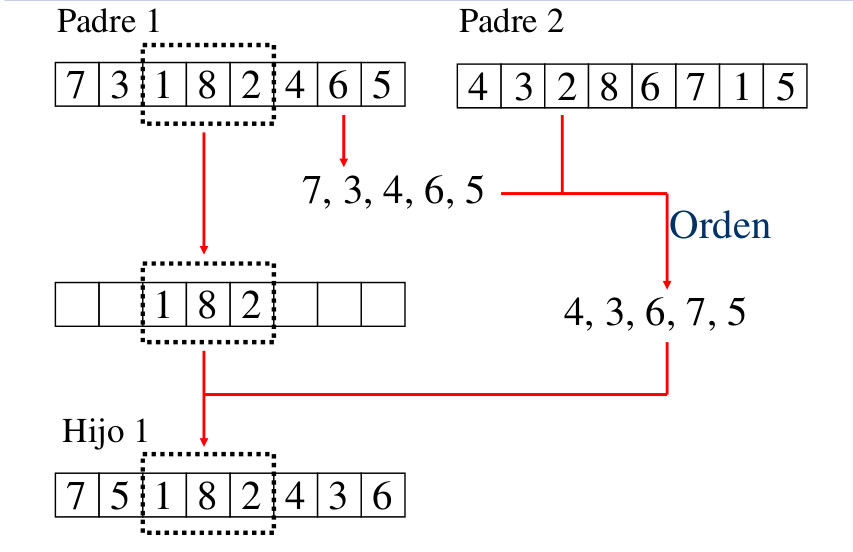
\includegraphics[width=220px]{../images/crossover_ox.jpg}
\caption{Operador de Cruce OX2 \label{cruce_ox}}
\end{figure}


En primer lugar se elige un rango central de elementos del cromosoma que se mantendrán de los padres a los hijos. El resto de posiciones a los extremos de los hijos se rellenan con la información del otro padre. Para ello, se van rellenando las posiciones de principio a fin en el mismo orden que en el padre.

\begin{figure}[ht!]
\centering
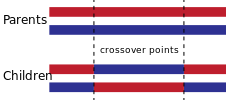
\includegraphics[width=220px]{../images/TwoPointCrossover}
\caption{Detalle operador de Cruce OX2 \label{cruce_ox_2}}
\end{figure}


\subsubsection{Operador de Mutación}

\bigskip
El \textbf{operador de mutación} intercambia entre dos elementos de la permutación. De forma aleatoria se elige si se mutará cada uno de los hijos con una probabilidad de mutación. La probabilidad de mutación son dos parámetro de nuestro algoritmo, probabilidad por individuo y probabilidad por gen, así que pueden modificar para tratar de mejorar las soluciones.

\subsubsection{Operador de Vecino}

\subsection{Técnicas de optimización local}

\bigskip
La técnica de optimización local utilizada es una técnica \textit{2-opt} proporcionada por el profesor. En la que se va comprobando como un intercambio de genes en un individuo puede mejorar su coste asociado. El pseudo-código de esta optimización es:

\begin{lstlisting}
S = candidato inicial con coste c(S) 
do {
	mejor = S
	for i=1..n
		for j=i+1..n
			T = S tras intercambiar i con j 
			if c(T) < c(S)
				S=T
} while (S != mejor)
\end{lstlisting}

\subsection{Algoritmo Genético Estándar}

En primer lugar se ha implementado un algoritmo genético básico, que utiliza los operadores de selección, cruce y mutación explicados anteriormente. Este algoritmo permite, al igual que los dos siguientes, que se indiquen un número de generaciones. El algoritmo acabará después de un número de generaciones especificado.


\subsection{Algoritmo Genético variante Baldwiniana}

La diferencia de esta variante respecto a la estándar es que se aplica una optimización local a cada generación. La optimización local se aplica una vez obtenida la nueva generación (a partir de los hijos) a todos los individuos. Una vez aplicada, se guarda el mejor individuo obtenido después de la optimización. Las soluciones optimizadas \textbf{no} se usan para generar la siguiente generación.

\subsection{Algoritmo Genético variante Lamarckiana}

La única diferencia de esta variante respecto a la \texttt{Baldwininana} es que las soluciones optimizadas, en este caso, \textbf{si} se usan para generar la siguiente generación.


\subsection{Parametros}

Los parámetros que podemos ajustar son los siguentes:

\begin{itemize}

	\item \textbf{Tamaño de población}: Una población que contiene \textbf{n} soluciones al problema. Dicha población va mejorando sus soluciones generación a generación.
	\item \textbf{Número de generaciones}: Numero de veces que va a "evolucionar' nuestra población.
	\item \textbf{Número de individuos en el torneo}: El número de elementos aleatorios que se obtendrán de la población para luego extraer el mejor de ellos. 
	\item \textbf{Probabilidad de mutación del individuo}: Aunque la mutación puede ayudar a dar más variedad a la población siempre puede provocar que no se explore a fondo un espacio donde podría haber una buena solución.
	\item \textbf{Probabilidad de mutación del gen}: Una vez se comprueba si un individuo muta se vuelve a comprobar por cada gen si este muta por otro. Este número debe ser bajo ya que si no se generarían individuos muy diferentes.
\end{itemize}



\chapter{Resultados}

Tras probar diferentes ajustes he detectado que había `sobreaprendizaje', esto es que aunque se mejora mucho el resultado para el conjunto de entrenamiento, a la hora de aplicar lo aprendido sobre el conjunto de prueba diera malos resultados. Tras ir ajustando los parámetros de las diferentes capas añadidas así como el número de neuronas se ha alcanzado una solución que daba unos resultados mas similares entre ambos conjuntos, siendo por tanto esta solución mucho mejor que un resultado dispar.

\bigskip
Los resultados obtenidos tras diversos ajustes en el algoritmo son bastante buenos, pasamos a detallarlos:

\begin{table}[H]
\centering

\begin{tabular}{|l|r|}
\hline
Tiempo de entrenamiento (en segundos)                 & 187  \\ \hline
Tasa de error sobre el conjunto de entrenamiento (\%) & 0.05  \\ \hline
Precisión sobre el conjunto de entrenamiento (\%)     & 99.95 \\ \hline
Tasa de error sobre el conjunto de prueba (\%)        & 0.64  \\ \hline
Precisión sobre el conjunto de prueba (\%)            & 99.36 \\ \hline
\end{tabular}
\caption{Tabla de resultados}

\end{table}

En la figura \ref{fig:plot} podemos ver como ha ido bajando el porcentaje de error en cada lote.

\begin{figure}[H]
\centering
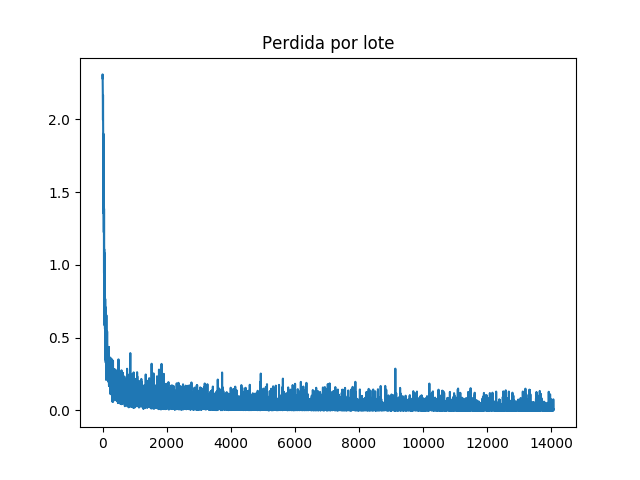
\includegraphics[width=1.0\textwidth]{../images/plot}
\label{fig:plot}
\end{figure}



\chapter{Conclusiones}

La realización de esta práctica me ha servido como introducción al basto mundo de las redes neuronales. Como nos comentó el profesor, necesitaríamos mucho mas tiempo que un simple cuatrimestre para profundizar mas, pues es un  campo muy amplio. Aun así ha sido muy gratificante poner a prueba los conocimientos adquiridos en la clase de teoría y viendo como los algoritmos van aprendiendo a resolver el problema de forma automática.

\bigskip
Aunque en un principio barajé la posibilidad de realizar una implementación por mi mismo, la falta de tiempo por motivos tanto laborales como académicos me lo ha impedido. De ahí a utilizar la librería Keras con TensorFlow como \textit{backend}. El poder utilizar una máquina en Amazon AWS con varias GPU me ha facilitado el poder probar en horas diferentes configuraciones que en mi máquina me hubiera llevado semanas a costa del desembolso económico.


\chapter{Anexos}
\section{Resultados de la ejecución}
\begin{lstlisting}
run:
-------------
Type: STANDARD
Solution: [9, 6, 8, 0, 7, 4, 1, 5, 2, 10, 3, 11]
Fitness: 11560
Problem size: 12
Population size: 100
Number of generations: 400
Individual mutation probability: 0.3
Gene mutation probability: 0.002
Tournament size: 4
Difference from optimal solution: 21.02177554438861%
Time: 1
Name:data/chr12a.dat
-------------
Type: STANDARD
Solution: [9, 4, 0, 7, 6, 10, 1, 5, 11, 3, 8, 2]
Fitness: 15582
Problem size: 12
Population size: 100
Number of generations: 400
Individual mutation probability: 0.3
Gene mutation probability: 0.002
Tournament size: 4
Difference from optimal solution: 63.12814070351759%
Time: 1
Name:data/chr12a.dat
-------------
Type: BALDWINIAN
Solution: [8, 11, 6, 4, 10, 7, 1, 2, 0, 5, 3, 9]
Fitness: 9552
Problem size: 12
Population size: 100
Number of generations: 400
Individual mutation probability: 0.3
Gene mutation probability: 0.002
Tournament size: 4
Difference from optimal solution: 0.0%
Time: 7
Name:data/chr12a.dat
-------------
Type: BALDWINIAN
Solution: [9, 0, 2, 8, 6, 4, 11, 3, 7, 5, 1, 10]
Fitness: 9552
Problem size: 12
Population size: 100
Number of generations: 400
Individual mutation probability: 0.3
Gene mutation probability: 0.002
Tournament size: 4
Difference from optimal solution: 0.0%
Time: 6
Name:data/chr12a.dat
-------------
Type: LAMARCKIAN
Solution: [6, 4, 11, 1, 0, 2, 8, 10, 9, 5, 7, 3]
Fitness: 9552
Problem size: 12
Population size: 100
Number of generations: 400
Individual mutation probability: 0.3
Gene mutation probability: 0.002
Tournament size: 4
Difference from optimal solution: 0.0%
Time: 5
Name:data/chr12a.dat
-------------
Type: LAMARCKIAN
Solution: [6, 4, 11, 1, 0, 2, 8, 10, 9, 5, 7, 3]
Fitness: 9552
Problem size: 12
Population size: 100
Number of generations: 400
Individual mutation probability: 0.3
Gene mutation probability: 0.002
Tournament size: 4
Difference from optimal solution: 0.0%
Time: 5
Name:data/chr12a.dat
-------------
Type: STANDARD
Solution: [1, 0, 7, 2, 9, 6, 10, 8, 4, 5, 3, 11]
Fitness: 586
Problem size: 12
Population size: 100
Number of generations: 400
Individual mutation probability: 0.3
Gene mutation probability: 0.002
Tournament size: 4
Difference from optimal solution: 1.384083044982699%
Time: 0
Name:data/nug12.dat
-------------
Type: STANDARD
Solution: [4, 5, 11, 3, 9, 10, 6, 7, 1, 8, 2, 0]
Fitness: 600
Problem size: 12
Population size: 100
Number of generations: 400
Individual mutation probability: 0.3
Gene mutation probability: 0.002
Tournament size: 4
Difference from optimal solution: 3.8062283737024223%
Time: 1
Name:data/nug12.dat
-------------
Type: BALDWINIAN
Solution: [0, 5, 10, 11, 3, 1, 4, 9, 6, 8, 7, 2]
Fitness: 578
Problem size: 12
Population size: 100
Number of generations: 400
Individual mutation probability: 0.3
Gene mutation probability: 0.002
Tournament size: 4
Difference from optimal solution: 0.0%
Time: 6
Name:data/nug12.dat
-------------
Type: BALDWINIAN
Solution: [10, 8, 7, 2, 1, 11, 6, 3, 5, 0, 9, 4]
Fitness: 578
Problem size: 12
Population size: 100
Number of generations: 400
Individual mutation probability: 0.3
Gene mutation probability: 0.002
Tournament size: 4
Difference from optimal solution: 0.0%
Time: 7
Name:data/nug12.dat
-------------
Type: LAMARCKIAN
Solution: [11, 6, 8, 2, 3, 7, 10, 0, 4, 5, 9, 1]
Fitness: 578
Problem size: 12
Population size: 100
Number of generations: 400
Individual mutation probability: 0.3
Gene mutation probability: 0.002
Tournament size: 4
Difference from optimal solution: 0.0%
Time: 3
Name:data/nug12.dat
-------------
Type: LAMARCKIAN
Solution: [4, 5, 9, 1, 3, 7, 10, 0, 11, 6, 8, 2]
Fitness: 578
Problem size: 12
Population size: 100
Number of generations: 400
Individual mutation probability: 0.3
Gene mutation probability: 0.002
Tournament size: 4
Difference from optimal solution: 0.0%
Time: 3
Name:data/nug12.dat
-------------
Type: STANDARD
Solution: [15, 8, 13, 17, 2, 10, 7, 11, 9, 0, 3, 19, 14, 1, 6, 16, 12, 18, 4, 5]
Fitness: 2656
Problem size: 20
Population size: 100
Number of generations: 400
Individual mutation probability: 0.3
Gene mutation probability: 0.002
Tournament size: 4
Difference from optimal solution: 3.3463035019455254%
Time: 0
Name:data/nug20.dat
-------------
Type: STANDARD
Solution: [16, 17, 4, 9, 5, 18, 1, 13, 0, 2, 3, 6, 11, 10, 12, 19, 14, 7, 15, 8]
Fitness: 2700
Problem size: 20
Population size: 100
Number of generations: 400
Individual mutation probability: 0.3
Gene mutation probability: 0.002
Tournament size: 4
Difference from optimal solution: 5.058365758754864%
Time: 0
Name:data/nug20.dat
-------------
Type: BALDWINIAN
Solution: [7, 17, 18, 0, 2, 16, 1, 5, 14, 9, 3, 12, 10, 19, 6, 15, 4, 11, 13, 8]
Fitness: 2570
Problem size: 20
Population size: 100
Number of generations: 400
Individual mutation probability: 0.3
Gene mutation probability: 0.002
Tournament size: 4
Difference from optimal solution: 0.0%
Time: 45
Name:data/nug20.dat
-------------
Type: BALDWINIAN
Solution: [3, 0, 9, 18, 11, 16, 2, 7, 13, 15, 19, 5, 6, 17, 12, 4, 1, 14, 10, 8]
Fitness: 2570
Problem size: 20
Population size: 100
Number of generations: 400
Individual mutation probability: 0.3
Gene mutation probability: 0.002
Tournament size: 4
Difference from optimal solution: 0.0%
Time: 42
Name:data/nug20.dat
-------------
Type: LAMARCKIAN
Solution: [16, 4, 6, 0, 5, 18, 14, 19, 7, 12, 3, 1, 11, 10, 15, 17, 13, 9, 2, 8]
Fitness: 2570
Problem size: 20
Population size: 100
Number of generations: 400
Individual mutation probability: 0.3
Gene mutation probability: 0.002
Tournament size: 4
Difference from optimal solution: 0.0%
Time: 32
Name:data/nug20.dat
-------------
Type: LAMARCKIAN
Solution: [17, 13, 9, 2, 8, 3, 1, 11, 10, 15, 18, 14, 19, 7, 12, 16, 4, 6, 0, 5]
Fitness: 2570
Problem size: 20
Population size: 100
Number of generations: 400
Individual mutation probability: 0.3
Gene mutation probability: 0.002
Tournament size: 4
Difference from optimal solution: 0.0%
Time: 29
Name:data/nug20.dat
-------------
Type: STANDARD
Solution: [16, 17, 5, 18, 10, 3, 1, 2, 13, 19, 4, 12, 14, 11, 8, 7, 15, 6, 0, 9]
Fitness: 3174
Problem size: 20
Population size: 100
Number of generations: 400
Individual mutation probability: 0.3
Gene mutation probability: 0.002
Tournament size: 4
Difference from optimal solution: 44.799270072992705%
Time: 0
Name:data/chr20a.dat
-------------
Type: STANDARD
Solution: [13, 3, 18, 12, 5, 11, 15, 0, 1, 17, 9, 6, 8, 10, 19, 16, 2, 4, 7, 14]
Fitness: 3466
Problem size: 20
Population size: 100
Number of generations: 400
Individual mutation probability: 0.3
Gene mutation probability: 0.002
Tournament size: 4
Difference from optimal solution: 58.120437956204384%
Time: 0
Name:data/chr20a.dat
-------------
Type: BALDWINIAN
Solution: [2, 4, 0, 7, 6, 1, 10, 16, 18, 13, 3, 8, 14, 15, 19, 9, 11, 5, 12, 17]
Fitness: 2244
Problem size: 20
Population size: 100
Number of generations: 400
Individual mutation probability: 0.3
Gene mutation probability: 0.002
Tournament size: 4
Difference from optimal solution: 2.3722627737226274%
Time: 67
Name:data/chr20a.dat
-------------
Type: BALDWINIAN
Solution: [14, 3, 4, 15, 6, 13, 18, 19, 11, 10, 7, 8, 0, 17, 12, 16, 2, 5, 1, 9]
Fitness: 2368
Problem size: 20
Population size: 100
Number of generations: 400
Individual mutation probability: 0.3
Gene mutation probability: 0.002
Tournament size: 4
Difference from optimal solution: 8.02919708029197%
Time: 47
Name:data/chr20a.dat
-------------
Type: LAMARCKIAN
Solution: [4, 10, 12, 17, 8, 1, 18, 16, 9, 19, 0, 3, 14, 7, 11, 2, 13, 15, 5, 6]
Fitness: 2196
Problem size: 20
Population size: 100
Number of generations: 400
Individual mutation probability: 0.3
Gene mutation probability: 0.002
Tournament size: 4
Difference from optimal solution: 0.18248175182481752%
Time: 35
Name:data/chr20a.dat
-------------
Type: LAMARCKIAN
Solution: [4, 10, 12, 17, 8, 1, 18, 16, 9, 19, 0, 3, 14, 7, 2, 11, 13, 15, 6, 5]
Fitness: 2196
Problem size: 20
Population size: 100
Number of generations: 400
Individual mutation probability: 0.3
Gene mutation probability: 0.002
Tournament size: 4
Difference from optimal solution: 0.18248175182481752%
Time: 32
Name:data/chr20a.dat
-------------
Type: STANDARD
Solution: [25, 22, 10, 3, 6, 24, 2, 15, 14, 0, 17, 11, 18, 19, 1, 20, 8, 13, 4, 12, 5, 7, 23, 21, 16, 9]
Fitness: 5438534
Problem size: 26
Population size: 100
Number of generations: 400
Individual mutation probability: 0.3
Gene mutation probability: 0.002
Tournament size: 4
Difference from optimal solution: 0.21862394433418653%
Time: 0
Name:data/bur26a.dat
-------------
Type: STANDARD
Solution: [11, 3, 10, 22, 13, 24, 14, 25, 8, 0, 17, 19, 7, 6, 1, 23, 4, 18, 20, 21, 2, 5, 15, 12, 9, 16]
Fitness: 5466197
Problem size: 26
Population size: 100
Number of generations: 400
Individual mutation probability: 0.3
Gene mutation probability: 0.002
Tournament size: 4
Difference from optimal solution: 0.7283840734741563%
Time: 0
Name:data/bur26a.dat
-------------
Type: BALDWINIAN
Solution: [7, 24, 22, 18, 0, 25, 11, 14, 3, 20, 23, 9, 4, 5, 19, 2, 13, 10, 12, 16, 21, 1, 15, 8, 6, 17]
Fitness: 5426670
Problem size: 26
Population size: 100
Number of generations: 400
Individual mutation probability: 0.3
Gene mutation probability: 0.002
Tournament size: 4
Difference from optimal solution: 0.0%
Time: 148
Name:data/bur26a.dat
-------------
Type: BALDWINIAN
Solution: [2, 7, 9, 21, 5, 12, 1, 11, 24, 18, 19, 4, 0, 20, 15, 22, 10, 14, 16, 8, 6, 17, 23, 3, 25, 13]
Fitness: 5426670
Problem size: 26
Population size: 100
Number of generations: 400
Individual mutation probability: 0.3
Gene mutation probability: 0.002
Tournament size: 4
Difference from optimal solution: 0.0%
Time: 132
Name:data/bur26a.dat
-------------
Type: LAMARCKIAN
Solution: [25, 10, 14, 6, 3, 12, 11, 5, 1, 17, 0, 8, 4, 20, 7, 13, 2, 18, 19, 24, 9, 16, 15, 23, 22, 21]
Fitness: 5426670
Problem size: 26
Population size: 100
Number of generations: 400
Individual mutation probability: 0.3
Gene mutation probability: 0.002
Tournament size: 4
Difference from optimal solution: 0.0%
Time: 79
Name:data/bur26a.dat
-------------
Type: LAMARCKIAN
Solution: [10, 14, 25, 6, 3, 12, 11, 5, 1, 17, 8, 4, 0, 20, 7, 13, 2, 18, 19, 9, 16, 24, 23, 15, 22, 21]
Fitness: 5426670
Problem size: 26
Population size: 100
Number of generations: 400
Individual mutation probability: 0.3
Gene mutation probability: 0.002
Tournament size: 4
Difference from optimal solution: 0.0%
Time: 84
Name:data/bur26a.dat
-------------
Type: STANDARD
Solution: [10, 12, 1, 22, 5, 3, 24, 20, 14, 0, 6, 18, 19, 17, 13, 15, 2, 8, 4, 7, 25, 9, 21, 11, 23, 16]
Fitness: 3826489
Problem size: 26
Population size: 100
Number of generations: 400
Individual mutation probability: 0.3
Gene mutation probability: 0.002
Tournament size: 4
Difference from optimal solution: 0.22622668453360686%
Time: 0
Name:data/bur26b.dat
-------------
Type: STANDARD
Solution: [22, 13, 21, 9, 5, 25, 3, 14, 20, 0, 19, 17, 18, 6, 15, 24, 2, 4, 8, 1, 11, 10, 12, 7, 23, 16]
Fitness: 3826071
Problem size: 26
Population size: 100
Number of generations: 400
Individual mutation probability: 0.3
Gene mutation probability: 0.002
Tournament size: 4
Difference from optimal solution: 0.2152781197385336%
Time: 1
Name:data/bur26b.dat
-------------
Type: BALDWINIAN
Solution: [20, 8, 10, 3, 18, 4, 1, 0, 23, 24, 5, 16, 12, 22, 21, 9, 2, 19, 15, 25, 6, 11, 14, 7, 17, 13]
Fitness: 3817852
Problem size: 26
Population size: 100
Number of generations: 400
Individual mutation probability: 0.3
Gene mutation probability: 0.002
Tournament size: 4
Difference from optimal solution: 0.0%
Time: 131
Name:data/bur26b.dat
-------------
Type: BALDWINIAN
Solution: [21, 8, 19, 9, 12, 15, 1, 11, 22, 5, 24, 23, 4, 16, 18, 0, 10, 20, 14, 2, 13, 3, 25, 7, 6, 17]
Fitness: 3817852
Problem size: 26
Population size: 100
Number of generations: 400
Individual mutation probability: 0.3
Gene mutation probability: 0.002
Tournament size: 4
Difference from optimal solution: 0.0%
Time: 117
Name:data/bur26b.dat
-------------
Type: LAMARCKIAN
Solution: [14, 24, 10, 6, 3, 1, 12, 21, 22, 17, 4, 0, 8, 20, 7, 11, 2, 18, 19, 16, 25, 9, 23, 15, 5, 13]
Fitness: 3817852
Problem size: 26
Population size: 100
Number of generations: 400
Individual mutation probability: 0.3
Gene mutation probability: 0.002
Tournament size: 4
Difference from optimal solution: 0.0%
Time: 105
Name:data/bur26b.dat
-------------
Type: LAMARCKIAN
Solution: [9, 24, 14, 6, 3, 1, 12, 21, 22, 17, 8, 0, 4, 20, 7, 11, 2, 18, 19, 10, 25, 16, 23, 15, 13, 5]
Fitness: 3817852
Problem size: 26
Population size: 100
Number of generations: 400
Individual mutation probability: 0.3
Gene mutation probability: 0.002
Tournament size: 4
Difference from optimal solution: 0.0%
Time: 100
Name:data/bur26b.dat
Error opening file: data/lipa40.dat (No such file or directory)
-------------
Type: STANDARD
Solution: [5, 15, 0, 9, 25, 21, 12, 3, 7, 20, 2, 13, 4, 8, 14, 6, 17, 19, 18, 22, 1, 23, 16, 24, 10, 11]
Fitness: 3840736
Problem size: 26
Population size: 100
Number of generations: 400
Individual mutation probability: 0.3
Gene mutation probability: 0.002
Tournament size: 4
Difference from optimal solution: 705.8936466204066%
Time: 0
Name:data/lipa40.dat
Error opening file: data/lipa40.dat (No such file or directory)
-------------
Type: STANDARD
Solution: [12, 22, 9, 11, 17, 15, 24, 7, 0, 25, 3, 19, 18, 2, 5, 14, 8, 20, 4, 10, 1, 21, 23, 13, 16, 6]
Fitness: 3831979
Problem size: 26
Population size: 100
Number of generations: 400
Individual mutation probability: 0.3
Gene mutation probability: 0.002
Tournament size: 4
Difference from optimal solution: 704.0561835238921%
Time: 0
Name:data/lipa40.dat
Error opening file: data/lipa40.dat (No such file or directory)
-------------
Type: BALDWINIAN
Solution: [0, 14, 4, 18, 13, 6, 10, 11, 12, 15, 16, 25, 20, 9, 19, 23, 2, 22, 7, 17, 5, 8, 24, 3, 21, 1]
Fitness: 3817852
Problem size: 26
Population size: 100
Number of generations: 400
Individual mutation probability: 0.3
Gene mutation probability: 0.002
Tournament size: 4
Difference from optimal solution: 701.0919444963185%
Time: 161
Name:data/lipa40.dat
Error opening file: data/lipa40.dat (No such file or directory)
-------------
Type: BALDWINIAN
Solution: [24, 20, 4, 9, 22, 10, 0, 14, 11, 5, 8, 21, 23, 1, 12, 6, 3, 18, 19, 7, 2, 16, 25, 15, 13, 17]
Fitness: 3817852
Problem size: 26
Population size: 100
Number of generations: 400
Individual mutation probability: 0.3
Gene mutation probability: 0.002
Tournament size: 4
Difference from optimal solution: 701.0919444963185%
Time: 122
Name:data/lipa40.dat
Error opening file: data/lipa40.dat (No such file or directory)
-------------
Type: LAMARCKIAN
Solution: [25, 9, 16, 6, 3, 1, 12, 21, 22, 17, 0, 8, 4, 20, 7, 11, 2, 18, 19, 24, 10, 14, 23, 15, 5, 13]
Fitness: 3817852
Problem size: 26
Population size: 100
Number of generations: 400
Individual mutation probability: 0.3
Gene mutation probability: 0.002
Tournament size: 4
Difference from optimal solution: 701.0919444963185%
Time: 106
Name:data/lipa40.dat
Error opening file: data/lipa40.dat (No such file or directory)
-------------
Type: LAMARCKIAN
Solution: [25, 14, 9, 6, 3, 5, 13, 22, 21, 17, 0, 4, 8, 20, 7, 11, 2, 19, 18, 24, 16, 10, 23, 15, 12, 1]
Fitness: 3817852
Problem size: 26
Population size: 100
Number of generations: 400
Individual mutation probability: 0.3
Gene mutation probability: 0.002
Tournament size: 4
Difference from optimal solution: 701.0919444963185%
Time: 109
Name:data/lipa40.dat
-------------
Type: STANDARD
Solution: [9, 47, 12, 2, 57, 22, 13, 56, 51, 52, 34, 58, 1, 39, 3, 6, 36, 19, 49, 28, 10, 23, 32, 11, 41, 18, 43, 21, 24, 29, 50, 31, 30, 7, 0, 46, 48, 27, 14, 45, 33, 26, 25, 5, 37, 42, 15, 20, 55, 35, 8, 38, 16, 54, 4, 53, 40, 17, 59, 44]
Fitness: 7756658
Problem size: 60
Population size: 100
Number of generations: 400
Individual mutation probability: 0.3
Gene mutation probability: 0.002
Tournament size: 4
Difference from optimal solution: 7.642227366727718%
Time: 2
Name:data/tai60a.dat
-------------
Type: STANDARD
Solution: [55, 37, 2, 1, 17, 32, 51, 42, 11, 47, 45, 29, 19, 22, 56, 39, 28, 41, 10, 34, 52, 59, 49, 15, 50, 58, 7, 43, 40, 36, 25, 12, 14, 16, 57, 5, 27, 38, 23, 6, 0, 13, 54, 9, 18, 21, 26, 8, 24, 46, 33, 31, 35, 44, 48, 20, 53, 3, 4, 30]
Fitness: 7787154
Problem size: 60
Population size: 100
Number of generations: 400
Individual mutation probability: 0.3
Gene mutation probability: 0.002
Tournament size: 4
Difference from optimal solution: 8.065432484934004%
Time: 3
Name:data/tai60a.dat
-------------
Type: BALDWINIAN
Solution: [189, 92, 122, 206, 74, 251, 24, 66, 166, 218, 21, 179, 41, 136, 107, 81, 27, 232, 255, 17, 51, 109, 198, 70, 128, 215, 172, 64, 44, 181, 151, 130, 201, 46, 87, 159, 238, 84, 59, 63, 29, 168, 148, 104, 186, 39, 0, 203, 244, 117, 77, 98, 6, 94, 160, 229, 31, 115, 155, 157, 89, 224, 56, 191, 183, 36, 242, 209, 249, 194, 53, 111, 162, 236, 113, 119, 253, 153, 134, 227, 247, 10, 102, 192, 140, 3, 145, 221, 34, 212, 126, 49, 32, 75, 199, 190, 228, 170, 169, 142, 11, 108, 225, 167, 197, 234, 176, 121, 38, 132, 52, 68, 233, 20, 22, 214, 101, 13, 15, 103, 195, 133, 152, 226, 141, 99, 149, 180, 14, 138, 62, 116, 48, 144, 139, 123, 216, 61, 171, 135, 33, 35, 82, 164, 158, 217, 58, 45, 90, 37, 8, 235, 47, 202, 23, 42, 248, 161, 208, 72, 106, 19, 86, 80, 252, 185, 91, 243, 18, 240, 2, 222, 174, 112, 50, 69, 196, 65, 105, 156, 30, 114, 154, 187, 230, 110, 250, 57, 9, 163, 188, 28, 207, 85, 1, 127, 246, 125, 213, 131, 173, 95, 7, 204, 241, 254, 76, 193, 67, 118, 25, 96, 124, 120, 55, 137, 239, 205, 100, 210, 43, 178, 4, 40, 5, 220, 237, 16, 129, 146, 54, 231, 182, 143, 211, 147, 78, 88, 60, 177, 71, 93, 79, 150, 26, 97, 223, 73, 245, 184, 83, 175, 200, 12, 219, 165]
Fitness: 44980610
Problem size: 256
Population size: 100
Number of generations: 400
Individual mutation probability: 0.3
Gene mutation probability: 0.002
Tournament size: 4
Difference from optimal solution: 0.49445820123972467%
Time: 154404
Name:data/tai256c.dat
-------------
Type: LAMARCKIAN
Solution: [109, 77, 30, 86, 83, 120, 111, 246, 68, 65, 232, 25, 19, 34, 55, 137, 181, 116, 47, 48, 5, 72, 57, 105, 122, 251, 213, 189, 176, 7, 253, 152, 174, 228, 51, 53, 94, 211, 22, 149, 222, 10, 2, 184, 201, 101, 75, 157, 79, 215, 107, 129, 172, 17, 243, 234, 134, 194, 249, 90, 124, 131, 219, 112, 43, 169, 236, 225, 80, 179, 45, 98, 208, 167, 60, 40, 207, 155, 15, 204, 36, 159, 164, 161, 186, 103, 198, 142, 239, 240, 146, 28, 12, 209, 69, 156, 39, 85, 56, 160, 74, 141, 91, 23, 114, 14, 238, 128, 143, 247, 16, 32, 70, 216, 250, 178, 44, 202, 197, 42, 88, 190, 223, 61, 193, 9, 100, 224, 231, 254, 59, 183, 121, 92, 99, 37, 170, 50, 171, 195, 102, 148, 205, 220, 136, 95, 151, 46, 133, 154, 241, 49, 192, 153, 180, 13, 87, 81, 191, 244, 0, 97, 89, 227, 200, 187, 221, 73, 24, 96, 150, 230, 106, 67, 218, 252, 11, 130, 217, 20, 126, 166, 4, 104, 140, 145, 226, 206, 248, 110, 118, 245, 233, 132, 33, 52, 158, 27, 31, 64, 125, 203, 93, 63, 138, 144, 214, 162, 66, 117, 229, 196, 123, 188, 21, 62, 135, 84, 165, 3, 235, 139, 185, 115, 29, 8, 212, 71, 210, 113, 127, 199, 41, 182, 54, 242, 1, 108, 26, 173, 168, 255, 35, 163, 175, 78, 58, 18, 147, 38, 82, 177, 76, 237, 6, 119]
Fitness: 44922898
Problem size: 256
Population size: 100
Number of generations: 400
Individual mutation probability: 0.3
Gene mutation probability: 0.002
Tournament size: 4
Difference from optimal solution: 0.36551961699842717%
Time: 177372
Name:data/tai256c.dat
\end{lstlisting}


\section{Código fuente del algoritmo genético implementado en lenguaje Java}
\begin{lstlisting}[language=java,caption={Main.java},captionpos=b]
/*  
 *  Inteligencia computacional
 *  Master Profesional en Ingeniería Informática
 * 
 *  2018 Copyleft - All Wrongs Reserved
 *
 *  Ernesto Serrano <erseco@correo.ugr.es>
 * 
 */
package qap;

import java.util.LinkedHashMap;
import qap.Genetic.AlgorithmType;

/**
 * 
 * @author Ernesto Serrano
 */
public class Main {
    public static void main(String[] args) {

        LinkedHashMap<String, Integer> map = new LinkedHashMap<>();

        map.put("data/chr12a.dat", 9552);
        map.put("data/nug12.dat", 578);
        map.put("data/nug20.dat", 2570);
        map.put("data/chr20a.dat", 2192);
        map.put("data/bur26a.dat", 5426670);
        map.put("data/bur26b.dat", 3817852);
        map.put("data/lipa40a.dat", 31538);
        map.put("data/tai60a.dat", 7205962);
        map.put("data/tai256c.dat", 44759294);        
        
        map.entrySet().forEach((entry) -> {
            for (AlgorithmType type : AlgorithmType.values()) {

                // We do many test of every algorytm
                for (int i = 0; i < 2; i++) {

                    Genetic alg = new Genetic(type, entry.getKey());

                    long startTime = System.currentTimeMillis();
                    alg.execute(entry.getValue());
                    long endTime = System.currentTimeMillis();
                    
                    System.out.println("Time: " + (endTime - startTime) / 1000);
                    System.out.println("Name:" + entry.getKey());
                    
                }
            }
        }); 
    }
}
\end{lstlisting}
\begin{lstlisting}[language=java,caption={Genetic.java},captionpos=b]
/*  
 *  Inteligencia computacional
 *  Master Profesional en Ingeniería Informática
 * 
 *  2018 Copyleft - All Wrongs Reserved
 *
 *  Ernesto Serrano <erseco@correo.ugr.es>
 * 
 */
package qap;

import java.io.File;
import java.io.FileNotFoundException;
import java.util.ArrayList;
import java.util.Collections;
import java.util.HashSet;
import java.util.Random;
import java.util.Scanner;
import java.util.Set;

/**
 * 
 * @author Ernesto Serrano
 */
public class Genetic {
    
    public enum AlgorithmType {
        STANDARD, 
        BALDWINIAN, 
        LAMARCKIAN,
    }
    
    protected static ArrayList<ArrayList<Integer>> distance_matrix;
    
    protected static ArrayList<ArrayList<Integer>>  flow_matrix;
    
    protected static int PROBLEM_SIZE;
    
    protected static final int POPULATION_SIZE = 100;
    
    private static final int NUMBER_OF_GENERATIONS = 400;

    private static final double INDIVIDUAL_MUTATION_PROBABILITY = 0.3;

    private static final double GENE_MUTATION_PROBABILITY = 0.002;

    private static final int TOURNAMENT_SIZE = 4;

    private final AlgorithmType type;
        
    private ArrayList<Individual> population;
    
    public Genetic(AlgorithmType type, String path) {
        this.type = type;
        this.load(path);
        
        population = createPopulation(POPULATION_SIZE);
        calculateFitness(population, type);
    }
    
    private  ArrayList<Individual> createPopulation(int size)  {
        ArrayList<Individual> newPopulation = new ArrayList<>();
        for (int i = 0; i < size; i++)
            newPopulation.add(new Individual());
        return newPopulation;
    }
    
    private void calculateFitness(ArrayList<Individual> population, AlgorithmType type) {
        population.forEach((individual) -> {
            individual.calculateFitness(type);
        }); 
    }

    private void load(String path) {
        
        try (Scanner scanner = new Scanner(new File(path))) {
            PROBLEM_SIZE = scanner.nextInt();
            flow_matrix = new ArrayList<>();
            distance_matrix = new ArrayList<>();

            for (int i = 0; i < PROBLEM_SIZE; i++) {
                flow_matrix.add(new ArrayList<>());
                for (int j = 0; j < PROBLEM_SIZE; j++) {
                    flow_matrix.get(i).add(scanner.nextInt());
                }
            }

            for (int i = 0; i < PROBLEM_SIZE; i++) {
                distance_matrix.add(new ArrayList<>());
                for (int j = 0; j < PROBLEM_SIZE; j++) {
                    distance_matrix.get(i).add(scanner.nextInt());
                }
            }
        } catch (FileNotFoundException ex) {
            System.out.println("Error opening file: " + ex.getMessage());
        }

    }

    public void execute(int optimal) {
        for (int i = 0; i < NUMBER_OF_GENERATIONS; i++) {
            ArrayList<Individual> generation = createPopulation(POPULATION_SIZE);

            for (int j = 0; j < POPULATION_SIZE / 2; j++) {
                // Parents to crossover
                Individual parent1 = select();
                Individual parent2 = select();
                // cannot repeat parent
                while (parent1.getFitness() == parent2.getFitness()) {
                    parent2 = select();
                } 

                // Crossover, mutate and calculate fitness of generated children
                Individual[] children = crossover(parent1, parent2);

                mutate(children[0]);
                mutate(children[1]);

                // Insert children in new population
                generation.set(2 * j, new Individual(children[0]));
                generation.set(2 * j + 1, new Individual(children[1]));
            }
            generation.add(new Individual(Collections.min(population))); // preserve best individual
            
            calculateFitness(generation, type);

            population = generation; // Evolve into the new generation
            
            // Remove the worst individuals to maintain the population size
            Collections.sort(population);
            while(population.size() > POPULATION_SIZE)
                population.remove(population.size()-1);
            
            //System.out.println("\t " + i + ": fitness: " + Collections.min(population).getFitness());
            
        }
        System.out.println("-------------");
        System.out.println("Type: " + type.toString());
        System.out.println("Solution: " + Collections.min(population).toString());
        System.out.println("Fitness: " + Collections.min(population).getFitness());
        System.out.println("Problem size: " + PROBLEM_SIZE);
        System.out.println("Population size: " + POPULATION_SIZE);
        System.out.println("Number of generations: " + NUMBER_OF_GENERATIONS);
        System.out.println("Individual mutation probability: " + INDIVIDUAL_MUTATION_PROBABILITY);
        System.out.println("Gene mutation probability: " + GENE_MUTATION_PROBABILITY);
        System.out.println("Tournament size: " + TOURNAMENT_SIZE);
        System.out.println("Difference from optimal solution: " + ((((double) Collections.min(population).getFitness() - optimal) / optimal) * 100) + "%");
    
    }
  
    private Individual select() {

        ArrayList<Individual> tournament = new ArrayList<>();
        Collections.shuffle(population);

        for (int i = 0; i < TOURNAMENT_SIZE; i++)
            tournament.add(population.get(i));        

        // return that individual
        return Collections.min(tournament) ;
    }

    /**
     * OX Crossover operation
     * @param parent0 First parent
     * @param parent1 Second parent
     */
    private Individual[] crossover(Individual parent0, Individual parent1) {
        Random random = new Random();

        // Create children
        Individual[] children  = new Individual[2];
        children[0] = new Individual();
        children[1] = new Individual();

        // Generating positions to cut
        int position1, position2;
        position1 = random.nextInt(PROBLEM_SIZE);
        do {
            position2 = random.nextInt(PROBLEM_SIZE);
        } while (position1 == position2); // cannot repeat the same position

        // First must be lower than second
        if (position2 < position1) {
            int swap = position1;
            position1 = position2;
            position2 = swap;
        }

        // Sets for a quicker search if a number is already in the solution of a child
        Set<Integer> individualsInChildren0 = new HashSet<>();
        Set<Integer> individualsInChildren1 = new HashSet<>();

        // Copy between the positions the partial solution of each parent
        for (int i = position1; i < position2; i++) {
            // Children 0 copies from parent 0
            children[0].getSolution()[i] = parent0.getSolution()[i];
            individualsInChildren0.add(children[0].getSolution()[i]);
            // Children 1 copies from parent 1
            children[1].getSolution()[i] = parent1.getSolution()[i];
            individualsInChildren1.add(children[1].getSolution()[i]);
        }

        for (int i = 0; i < PROBLEM_SIZE; i++) { // iterate children
            if (i < position1 || i >= position2) { // not between the positions
                // Search for the first value in the parent 1 which is not currently in the child 0
                int iterator = 0;
                while (individualsInChildren0.contains(parent1.getSolution()[iterator])) {
                    iterator++;
                }
                // Children 0 copies from parent 1
                children[0].getSolution()[i] = parent1.getSolution()[iterator];
                individualsInChildren0.add(parent1.getSolution()[iterator]);

                // Search for the first value in the parent 1 which is not currently in the child 0
                iterator = 0;
                while (individualsInChildren1.contains(parent0.getSolution()[iterator])) {
                    iterator++;
                }
                // Children 1 copies from parent 0
                children[1].getSolution()[i] = parent0.getSolution()[iterator];
                individualsInChildren1.add(parent0.getSolution()[iterator]);
            }
        }

        return children;
    }

    private void mutate(Individual individual) {
        Random random = new Random();
        double prob = random.nextDouble();
        // Check if mutate
        if (prob < INDIVIDUAL_MUTATION_PROBABILITY) {
            for (int i = 0; i < PROBLEM_SIZE; i++) {
                prob = random.nextDouble();
                if (prob < GENE_MUTATION_PROBABILITY) {
                    // Position to mutate with i
                    int j;
                    do {
                        j = random.nextInt(PROBLEM_SIZE);
                    } while (j == i); // cannot mutate the same position
                    individual.swap(i, j); // mutate
                }
            }
        }
    }

}
\end{lstlisting}
\begin{lstlisting}[language=java,caption={Individual.java},captionpos=b]
/*  
 *  Inteligencia computacional
 *  Master Profesional en Ingeniería Informática
 * 
 *  2018 Copyleft - All Wrongs Reserved
 *
 *  Ernesto Serrano <erseco@correo.ugr.es>
 * 
 */
package qap;

import java.util.ArrayList;
import java.util.Arrays;
import java.util.Collections;
import java.util.Random;
import qap.Genetic.AlgorithmType;

/**
 * 
 * @author Ernesto Serrano
 */
public class Individual implements Comparable<Individual> {
        
    private int[] solution;

    private int fitness;
    
    public Individual() {
        this.solution = new int[Genetic.PROBLEM_SIZE];
        this.fitness = Integer.MAX_VALUE;
        this.generateRandomSolution();
    }

    public Individual(Individual source) {
        solution = new int[Genetic.PROBLEM_SIZE];
        System.arraycopy(source.solution, 0, solution, 0, source.solution.length);
        fitness = source.fitness;
    }

    public void calculateFitness(AlgorithmType algType) {
        switch (algType) {
            case LAMARCKIAN:
                calculateFitnesLamarckian();
                break;
            case BALDWINIAN:
                calculateFitnesBalwinian();
                break;
            default:
                calculateFitnesStandard();
        }
    }

    public void calculateFitnesStandard (){
        int newFitness = 0;
        for (int i = 0; i < Genetic.PROBLEM_SIZE; i++) {
            for (int j = 0; j < Genetic.PROBLEM_SIZE; j++) {                
                newFitness += Genetic.flow_matrix.get(i).get(j) * Genetic.distance_matrix.get(solution[i]).get(solution[j]);
            }
        }
        fitness = newFitness;
    }

    public void calculateFitnesLamarckian (){
        // Changes the current individual using the optimized individual values
        Individual optimized = greedy();
        solution = new int[Genetic.PROBLEM_SIZE];
        System.arraycopy(optimized.solution, 0, solution, 0, optimized.solution.length);
        fitness = optimized.fitness;
    }

    public void calculateFitnesBalwinian (){
        // Only changes the fitness using the optimized individual one
        Individual optimized = greedy();
        this.fitness = optimized.getFitness();
    }
    
    public int getFitness() {
        return fitness;
    }
    
    public int[] getSolution() {
        return solution;
    }

    public void swap(int pos1, int pos2) {
        int gene = solution[pos1];
        solution[pos1] = solution[pos2];
        solution[pos2] = gene;
    }

    private void generateRandomSolution() {
        
        // Initialize ordered list
        ArrayList<Integer> list = new ArrayList<>();
        for (int i = 0; i < Genetic.PROBLEM_SIZE; i++)
            list.add(i);

        // Shuffle list
        Collections.shuffle(list, new Random());
        
        // Copy to primitive array
        for (int i = 0; i < Genetic.PROBLEM_SIZE; i++) {
            solution[i] = list.get(i);
        }
                
        // Calculate fitness
        calculateFitness(AlgorithmType.STANDARD);
    }

    /**
     * Greedy 2-opt algorithm to optimize an individual
     */
    private Individual greedy() {
        Individual best;
        Individual S = new Individual(this);
        S.calculateFitnesStandard();
        do {
            best = new Individual(S); // save best solution by now
            for (int i = 0; i < solution.length; i++) {
                for (int j = i + 1; j < solution.length; j++) {
                    // Create T exchanging i and j gene
                    Individual T = new Individual(S);
                    T.solution[i] = S.solution[j];
                    T.solution[j] = S.solution[i];
                    
                    T.calculateFitnesStandard();
                    
                    if (T.getFitness() < S.getFitness()) { // if new solution is better than older updates
                        S = new Individual(T);
                    }
                }
            }
        } while (S.getFitness() < best.getFitness());
        return S;
    }
    
    @Override
    public String toString() {
        return Arrays.toString(this.solution);
    }
    
    @Override
    public int compareTo(Individual o) {
        return this.fitness - o.fitness;
    }
}
\end{lstlisting}

\newpage \
\thispagestyle{empty}
\end{document}